\documentclass[a4paper]{report}
\usepackage[utf8]{inputenc}
\usepackage[T1]{fontenc} 
\usepackage[francais]{babel}
\usepackage{graphicx}
\usepackage{geometry}
\usepackage{color}
\usepackage{fancyhdr}
\pagestyle{fancy}
\fancyhf{}
\lhead{2011/2012}
\rhead{IUT Nancy Charlemagne}
\geometry{hmargin=1cm,vmargin=2cm,lmargin=2cm,rmargin=2cm}
\lfoot{Mathieu LEROUX}
\cfoot{Projet tuteuré: Déduplication \\ Licence ASRALL}
\rfoot{\thepage}
\renewcommand{\footrulewidth}{2pt}
\begin{document}
	\chapter*{Déduplication}
	La déduplication de données est une technique qui permet de minimiser de l'espace de stockage. Elle consiste à ne pas répliquer les données déja existantes sur le disque. Un fichier est décomposé sous forme de blocs de données car des fichiers peuvent avoir des blocs en commum. Le mécanisme de déduplication crée une table avec les index de tous les blocs de données des fichiers présents sur le disque. La taille des blocs peut varier selon les mécanismes utilisés mais plus les blocs sont petits, plus il y aura de chance qu'un autre bloc soit identique et donc, plus la déduplication sera efficace. En général, cette taille ne dépasse pas les 128ko.
 
 Quand un utilisateur dépose un fichier, le mécanisme crée ses index et regarde s'il n'y a pas des blocs déjà existants. Si des blocs sont similaires alors une simple référence aux blocs déjà existants sera crée. Le schéma ci-dessous montre comment la déduplication fonctionne. Les blocs étant de la même couleur sont considérés identiques.\\
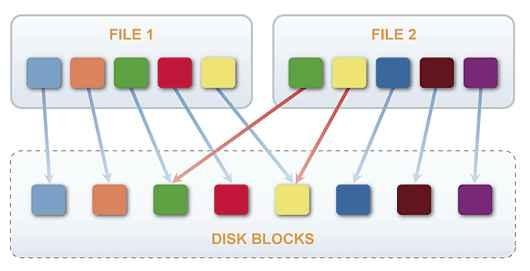
\includegraphics[width=10cm]{deduplication.jpg}

Il existe deux types de dépuplication: la déduplication à la volée (à la source) et la déduplication hors ligne (à la destination). La déduplication à la volée analyse les fichiers avant de les stocker pour savoir s'ils n'existent pas déjà sur le disque. Cette technique utilise une forte consommation CPU et mémoire. L'autre technique consiste à copier dans un premier temps le fichier sur le disque avant de tester s'il existe déjà. Cela nécessite de prévoir un espace de stockage tampon plus important. \\

Dans un contexte de serveur de messagerie et de fichiers centralisés, la déduplication de données peut très rapidement économiser de nombreux gigaoctets d'espace disque ainsi que la diminution de la bande passante qui aurait été utilisée pour la sauvegarde. En effet, dans le cas où un même mail de 1Mo est envoyé à cinquante destinataires alors l'économie du disque sera de 50-1 megaoctets (stockage d'un seul mail). La déduplication est faite pour des fichiers tels que des documents bureautiques ou des machines virtuelles qui ont souvent de nombreux blocs en commun.\\
Le terme inverse de la déduplication est la réhydratation. Elle fait appel à la table des index afin de renvoyer tous les blocs de données référencés pour un fichier demandé.\\

Certain outils comme LessFS mise en relation avec un système de fichiers ZFS permettent de dédupliquer et de compresser les blocs de données. Cela permet de gagner encore plus d'octets sur le disque mais nécessite une consommation mémoire et CPU plus importante.

	\chapter*{ZFS}
	\section{Introduction}
	Le système de fichier ZFS (Zettabyte File System) a été conçu par Sun en 2005 et est sous licence CDDL.  Il n'était disponible que sous Solaris mais est devenu récemment disponible sous linux. Il est l'un des systèmes de fichiers les plus intéressants du marché. En effet, ZFS intègre de nombreux avantages que d'autres n'ont pas. Voici une liste de ses principaux avantages: \\
	\begin{itemize}
		 \item Pas de limites pratiques (taille des disques, fichiers, ...)
		 \item Garantir la sécurité des données (intégrité, disponibilité)
		 \item Administration simplifiée
		 \item Gestionnaire de volume intégré
		 \item Compression
		 \item Snapshot
		 \item Duplication
		 \item Quotas et réservation d’espace
		 \item Performances élevées
		 \item Indépendant de l’architecture matérielle\\
	\end{itemize}
	ZFS est un système de fichier 128 bits contrairement aux autres systèmes qui sont de 64 bits. Ainsi ses limites sont de 16 milliards de milliards fois plus autant dire qu'il n'a quasi pas de limite. Afin d'optimiser ses performances, ZFS utilise tout l'espace disponible de la RAM pour créer un énorme cache. Ce procédé s'appelle ARC (Adaptive replacement cache). Il peut poser problème aux autres processus qui testent la mémoire inutilisée avant de ce lancer mais cette mémoire est souvent inutilisée. Il peut être partagé via le réseau avec d'autres systèmes de fichiers comme nfs ou samba. Ainsi même depuis des systèmes qui ne le supporte pas, il sera accessible.\\
	\section{Stockage}
	ZFS fonctionne avec un pool. C'est un ensemble de périphériques qui fournissent de l’espace pour le stockage et la duplication des données comme le raid logiciel. \\
	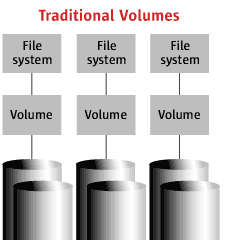
\includegraphics[width=5cm]{volumes_tradicionais.png}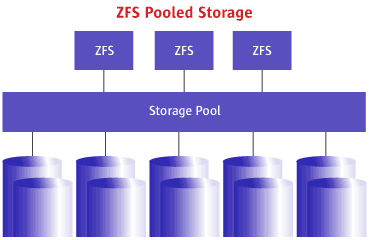
\includegraphics[width=7cm]{armazenamento_pooled_zfs.png}\\
	Voici les différentes unités de base de stockage de données :\\
	\begin{itemize}
		 \item Disques : entiers ou juste une partition
		 \item Fichiers dans un autre système de fichiers
		 \item Miroirs : 2 (ou plus) disques, partitions ou fichiers
		 \item Raid-z : plusieurs disques, variante de RAID-5\\
	\end{itemize}
	ZMirror est un miroir classique. Il utilise les mécanismes de checksum pour valider les lectures sur un composant et bascule sur le second s'il détecte une erreur puis corrige le composant défaillant (si possible). Le système Raid-z est similaire au procédé Raid 5. Il utilise les checksums (SHA-256 + fletcher) et repose sur le copy on write : supprime le "write-hole".

	\chapter*{Compression}
	Tout comme la déduplication, la compression est une technique qui permet d'économiser de l'espace de stockage. Chaque fichier est constitué d'une succession de millions de bits 0 ou 1. La compression permet de diminuer le nombre de bits que constitue un fichier en changeant la succession de bits de départ. Suivant l'algorithme de codage utilisé, le taux de compression peut différer. Les algorithmes d'encodage sont plus ou moins efficaces selon le type de fichier compressé.\\
 Il existe deux types de compression: la compression avec perte et sans perte. La compression sans perte signifie qu'après la décompression, le fichier sera identique au fichier compressé. C'est le plus souvent utilisé sur des documents, des fichiers exécutables ou des archives. Ces données étant principalement des caractères texte, ils ne peuvent pas être modifiés. Les formats de documentation tels que txt, doc ou pdf sont donc compressés sans perte.  Tant qu'à la compression avec perte, les fichiers décompressés ne seront pas exactement identiques au fichier original mais les informations seront sensiblement les mêmes. Les types de fichiers utilisés par cette compression sont les images, les sons et les vidéos. Cett technique se repose sur la limitation des sens de l'homme comme la vision et l'audition. L'homme ne pourra donc pas identifier les différences entre le fichier original et le fichier après décompressage. Les formats de fichiers jpeg, avi ou mp3 sont donc compressés avec pertes. \\
Pour chaque technique de compression, il existe plusieurs algorithmes de codage.\\
	\section{Compression sans perte}
	Parmi les algorithmes sans perte, il y a les algorithmes tels que Lempei-Ziv ou le codage RLE (Run-Length Encoding) qui consistent à remplacer des suites de bits utilisées plusieurs fois dans un même fichier. D'autres algorithmes comme l'algorithme de codage Huffman détermine les suites de bits et plus une suite est utilisée souvent, plus la suite qui la replacera sera courte.
	\subsection{L'algorithme Lempel-Ziv}
		Cet algorithme se divise en deux versions distinctes : LZ77 et LZ78. Ces algorithmes utilisent un dictionnaire où ils référencent les motifs récurrents. A la rencontre d'un motif du dictionnaire, une simple référence au motif est faite (fenêtre glissante). La déduplication utilise globalement le même procédé.\\
	\subsubsection{LZ77}
		La compression LZ77 encode avec un taux de compression inférieur à d'autres algorithmes comme PPM et CM (voir ci-dessous) mais a le double avantage d'être rapide et asymétrique. Cela lui permet d'utiliser un algorithme de décompression différent de celui de la compression. Ainsi, la compression pourra être rapide et la décompression performante. Les variantes LZSS et LZMA sont basées sur la compression LZ77 et supprime quelques inconvénients de celle-ci tels que le taux de compression assez faible (pour LZMA) ou le problème si aucun motif récurrent n'est rencontré (pour LZSS). Ce problème aura pour conséquence d'augmenter la taille du fichier. La compression LZ77 est la base des algorithmes comme Deflate (ZIP, gzip) et donc LZMA (7-zip).
	\subsubsection{LZ78}
		La compression LZ78 ou Lempel-Ziv-Welch utilise aussi un dictionnaire mais au lieu de le remplir au fur et à mesure des motifs rencontrés, il crée un dictionnaire initial de tous les symboles possibles. Cela permet d'améliorer la compression car les données du dictionnaire ne devant plus être envoyées au décompresseur, l'espace utilisé est réduit. L'utilisation de cette technique a été réduite jusque 2003 car elle a été brevetée par UNISYS qui n'avait pas laissé la licence libre.
	\subsubsection{LZO}
		Lempel-Ziv-Oberhumer (LZO) est un algorithme de compression en temps réel se basant sur les dictionnaires. Ces avantages sont une compression et décompression rapide. L'un des logiciels l'utilisant est lzop.
	\subsection{L'algorithme RLE}
		Le run-length encoding (codage par plages) est une technique de compression qui s'applique uniquement sur des documents scannés en noir et blanc tels que des fax. Elle consiste à factoriser les termes d'une même couleur. Ainsi la chaîne : NNNNNNNBBBBNNNNNNNNNNBB (N étant le nombre de points noirs et B étant le nombre de points blancs) sera encodée par RLE en : 7N4B10N2B . Les formats d'images utilisent cette compression en considérant que toutes les lignes de pixels sont jointes pour former une unique séquence de couleur. Les images BMP utilisent cette compression en 1,4 et 8 bits/pixel (noir et blanc, 16 couleurs et 256 couleurs). Le format PCX utilise aussi cette compression pour les images de 8 et 24 bits/pixels. Celles de 24 bits étant découpées en trois parties de 8 bits chacune.
	\subsection{Codage par modélisation de contexte}
	\subsubsection{Prédiction par reconnaissance partielle (PPM)}
		La prédiction par reconnaissance partielle se base sur une modélisation de contexte pour évaluer la probabilité des différents symboles. Le contexte est un ensemble de symboles déjà rencontrés dans la source de données. Elle utilise les données déjà analysées pour en déduire les données à analyser. Ainsi plus le contexte est long, meilleur sera la prédiction et donc la compression. La prédiction obtenue servira d'entrée à un codage entropique comme le codage Huffman. Elle a l'avantage d'être l'une des plus performantes sur la compression de fichiers texte mais a l'inconvénient de consommer énormément de mémoire si le contexte est très grand. La PPM est un algorithme symétrique contrairement à Lempel-Ziv ce qui signifie qu'il utilise le même pour la compression que pour la décompression. Cela implique un temps d'exécution identique et assez lent.
	\subsubsection{Pondération de contextes (CM)}
		La pondération de contextes consiste à utiliser plusieurs prédicteurs (par exemple des PPM) pour obtenir l'estimation la plus fiable possible du symbole à venir. A l'image de la prédiction par reconnaissance partielle, les taux de compressions sont très élevés mais proportionnellemnt aussi lents que la taille du contexte.
	\subsection{L'algorithme de codage Huffman}
		Cette compression s'apparente à la compression du code morse. Elle consiste donc à coder les séquences fréquentes sur peu de place et ce qui revient rarement sur des séquences plus longues. L'inconvénient avec ce procédé c'est qu'il faut avoir analysé tout le fichier pour créer une table avec les redondances avant de pouvoir le compresser. Il faut donc envoyer la table pour pouvoir le décompresser ce qui peut être problématique quand le fichier à compresser est petit. Le codage Huffman adaptatif corrige ce problème car il remplit au fur et à mesure la table et démarre la compression avec une table de base. \\
	Ce codage est utilisé en seconde compression après que le premier algorithme (tel que LZ77) est mis en évidence la redondance d'information. Ce codage peut être utilisé pour la compression tels que JPEG, MPEG ou MP3 où les données imperceptibles par l'homme sont supprimées mais on parle donc de compression avec pertes.
	\section{Compression avec pertes}
		La compression avec pertes s'utilisent donc sur des données perceptibles par l'homme comme les sons, les images ou les vidéos. Elles suppriment les données que l'homme ne perçoit pas ou quasiment pas. Ainsi pour le format JPEG 2000, la compression est de 1 bit/pixels au lieu de 24 bits/pixels. La compression avec pertes est une technique irréversible c'est à dire qu'il ne sera pas possible de retrouver le fichier original. Il existe trois grandes familles de compression avec pertes: la compression par prédiction, par transformation et la compression basée sur les récurrences fractales de motif.
	\subsection{Compression par prédiction}
		Cet algorithme repose sur un schéma de prédiction et un codage des erreurs entre la prédiction et le signal original. La prédiction consiste à prédire les données à venir en fonction des données analysées. Les erreurs étant souvent de faibles magnitudes, une compression intéressante est possible grâce à la diminution des bits nécessaires à l’opération. Certain formats de codecs de microsoft et d'Apple utilisent cette compression.
	\subsection{Compression par transformation}
		Cet algorithme transforme le signal en atténuant les fréquences non décelables par l'homme. Cette technique transforme donc le signal du domaine temporel au domaine fréquentiel afin de déterminer et de supprimer les pixels redondants.  Le schéma ci-dessous montre cette transformation.\\
	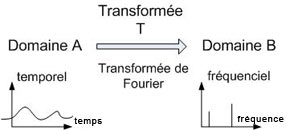
\includegraphics[width=5cm]{transformation.jpg} \\
La compression JPEG,JPEG 2000 ou encore MPEG utilise cette compression. Cette méthode de compression est la plus répandue au vue de ces performances.
	\subsubsection{La norme JPEG}
		La norme JPEG (Joint Photographic Experts Group) est une norme qui définit le format d'enregistrement et l'algorithme de décodage pour une représentation numérique compressée d'une image fixe. La norme JPEG peut être compressée sans perte mais son taux de compression n'est que de 2 au lieu de 3 à 100.
Le shéma ci-dessous montre ses étapes de compression et décompression.\\
		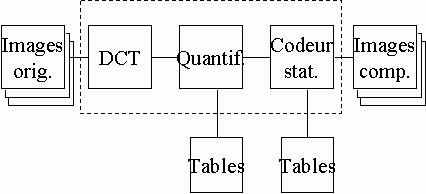
\includegraphics[width=10cm]{schema.jpg} \\
		Tout d'abord, le format JPEG commence par découper l'image en blocs de données comme beaucoup d'autres formats compressés avec pertes. Puis JPEG transforme les couleurs de chaque bloc à l'aide de la transformée DCT (transformée en cosinus discrète) assimilable à la transformée de Fourier qui transforme le signal temporel en signal fréquentiel (DCT). La valeur des fréquences résultantes détermineront leurs importances dans l'image. Une matrice de ces résultats sera générée. La quantification est l'étape qui permet de réduire considérablement la taille de l'image. En effet, elle utilise la DCT pour atténuer les fréquences non perceptibles par l'homme. La matrice résultante par la quantification sera ensuite codée par un algorithme RLE puis par un algorithme d'Huffman afin d'être compressée. Lors de la quantification et du codage, des tables sont créées et envoyées avec le fichier compressé pour la décompression.\\
	Lors de la compression du format JPEG sans perte, l'étape de la quantification n'est pas présente.

	\subsubsection{Compression par ondelette}
		La compression (ou transformée) par ondelette s'utilise globalement comme la norme JPEG mais génère une image de meilleure qualité avec un taux de compression supérieure (de 15 à 50). Contrairement à la transformée DCT, l'image est analysée plus finement et a un résultat plus proche de la perception humaine. Les codeurs JPEG 2000 et SPIHT utilisent tous deux une transformée en ondelettes dans leur schéma de compression. Les domaines d'utilisation de cette compression est l'imagerie médicale, les empreintes digitales ou encore dans le cinéma.

	\subsection{Compression basée sur les récurrences fractales de motif}
		La compression basée sur les récurrences fractales de motif aussi appelée compression fractale est utilisée pour la compression d'image. Son principe est de détecter les récurrences de motifs et de supprimer les informations redondantes de l'image. Plusieurs méthodes existent mais la plus connue est la méthode Jacquin. Deux étapes composent cette méthode. Dans un premier temps, deux segmentations sont réalisées: une segmentation de figure source et destination. Ensuite pour chaque figure Source, une figure destination est cherchée afin de créer un couple pour minimiser une erreur. Cette erreur est le résultat de leur soustraction après avoir dimensionné le couple de manière identique. A ce stade, des transformations comme la rotation peuvent être réalisées.
		
         
\end{document} 
